% ===============================================
% ANNEXES 
% ===============================================

\appendix

% ===============================================
% ANNEXE A
% ===============================================
\chapter{Tests préliminaires avec capteur inertiel} \label{ann:imu-tests}

Avant d'opter pour une approche purement basée sur la vision par ordinateur, une exploration initiale a été conduite avec un capteur inertiel (IMU) fixé directement sur la barre, dans le but de quantifier les paramètres cinématiques du mouvement (vitesse, rotation, trajectoire).

\section*{Matériel utilisé}

Le capteur utilisé est le \textbf{WIT WT9011DCL}, une centrale inertielle 9 axes combinant accéléromètre, gyroscope et magnétomètre, avec transmission Bluetooth vers un téléphone portable via l'application mobile propriétaire. Le capteur a été fixé à la barre via une bande velcro : une partie de la bande collée sur le boîtier du capteur, et l'autre partie enroulée autour de la barre, permettant un positionnement rapide et réversible sans abîmer l'équipement. La fréquence d'acquisition est de 200~Hz, produisant des enregistrements au format texte tabulé contenant les colonnes d'accélération (g), de vitesse angulaire (°/s), d'angles d'Euler (°), de champ magnétique ($\mu$T) et de quaternions d'orientation.

\section*{Métriques visées et pipeline de traitement}

L'objectif initial était de calculer trois paramètres cinématiques à partir des données brutes de l'IMU. Le traitement des données a été implémenté en Python via une classe \texttt{IMUProcessor} reposant sur les bibliothèques \texttt{pandas}, \texttt{numpy}, \texttt{scipy} et \texttt{matplotlib}. Les accélérations brutes exprimées dans le repère capteur sont d'abord converties dans le repère terrestre via les quaternions d'orientation fournis par le capteur (\texttt{sensor\_to\_earth}). Un biais gravitationnel est estimé sur les 2 premières secondes d'enregistrement (400 échantillons à 200~Hz) et soustrait. La vitesse est ensuite obtenue par intégration numérique de l'accélération, avec une correction de la dérive via \texttt{scipy.signal.detrend}. La rotation de la barre autour de son axe longitudinal est estimée via l'intégration des vitesses angulaires fournies par le gyroscope, après compensation du biais de repos calculé sur les premières mesures statiques. La trajectoire est obtenue par double intégration de l'accélération (intégration de la vitesse), avec une correction de la dérive appliquée sur chaque axe. Une visualisation 3D interactive de la trajectoire de la barre (figure~\ref{fig:imu-trajectory}) est générée via \texttt{matplotlib} avec une normalisation des axes pour éviter les distorsions de perspective.

\begin{figure}[h]
  \centering
  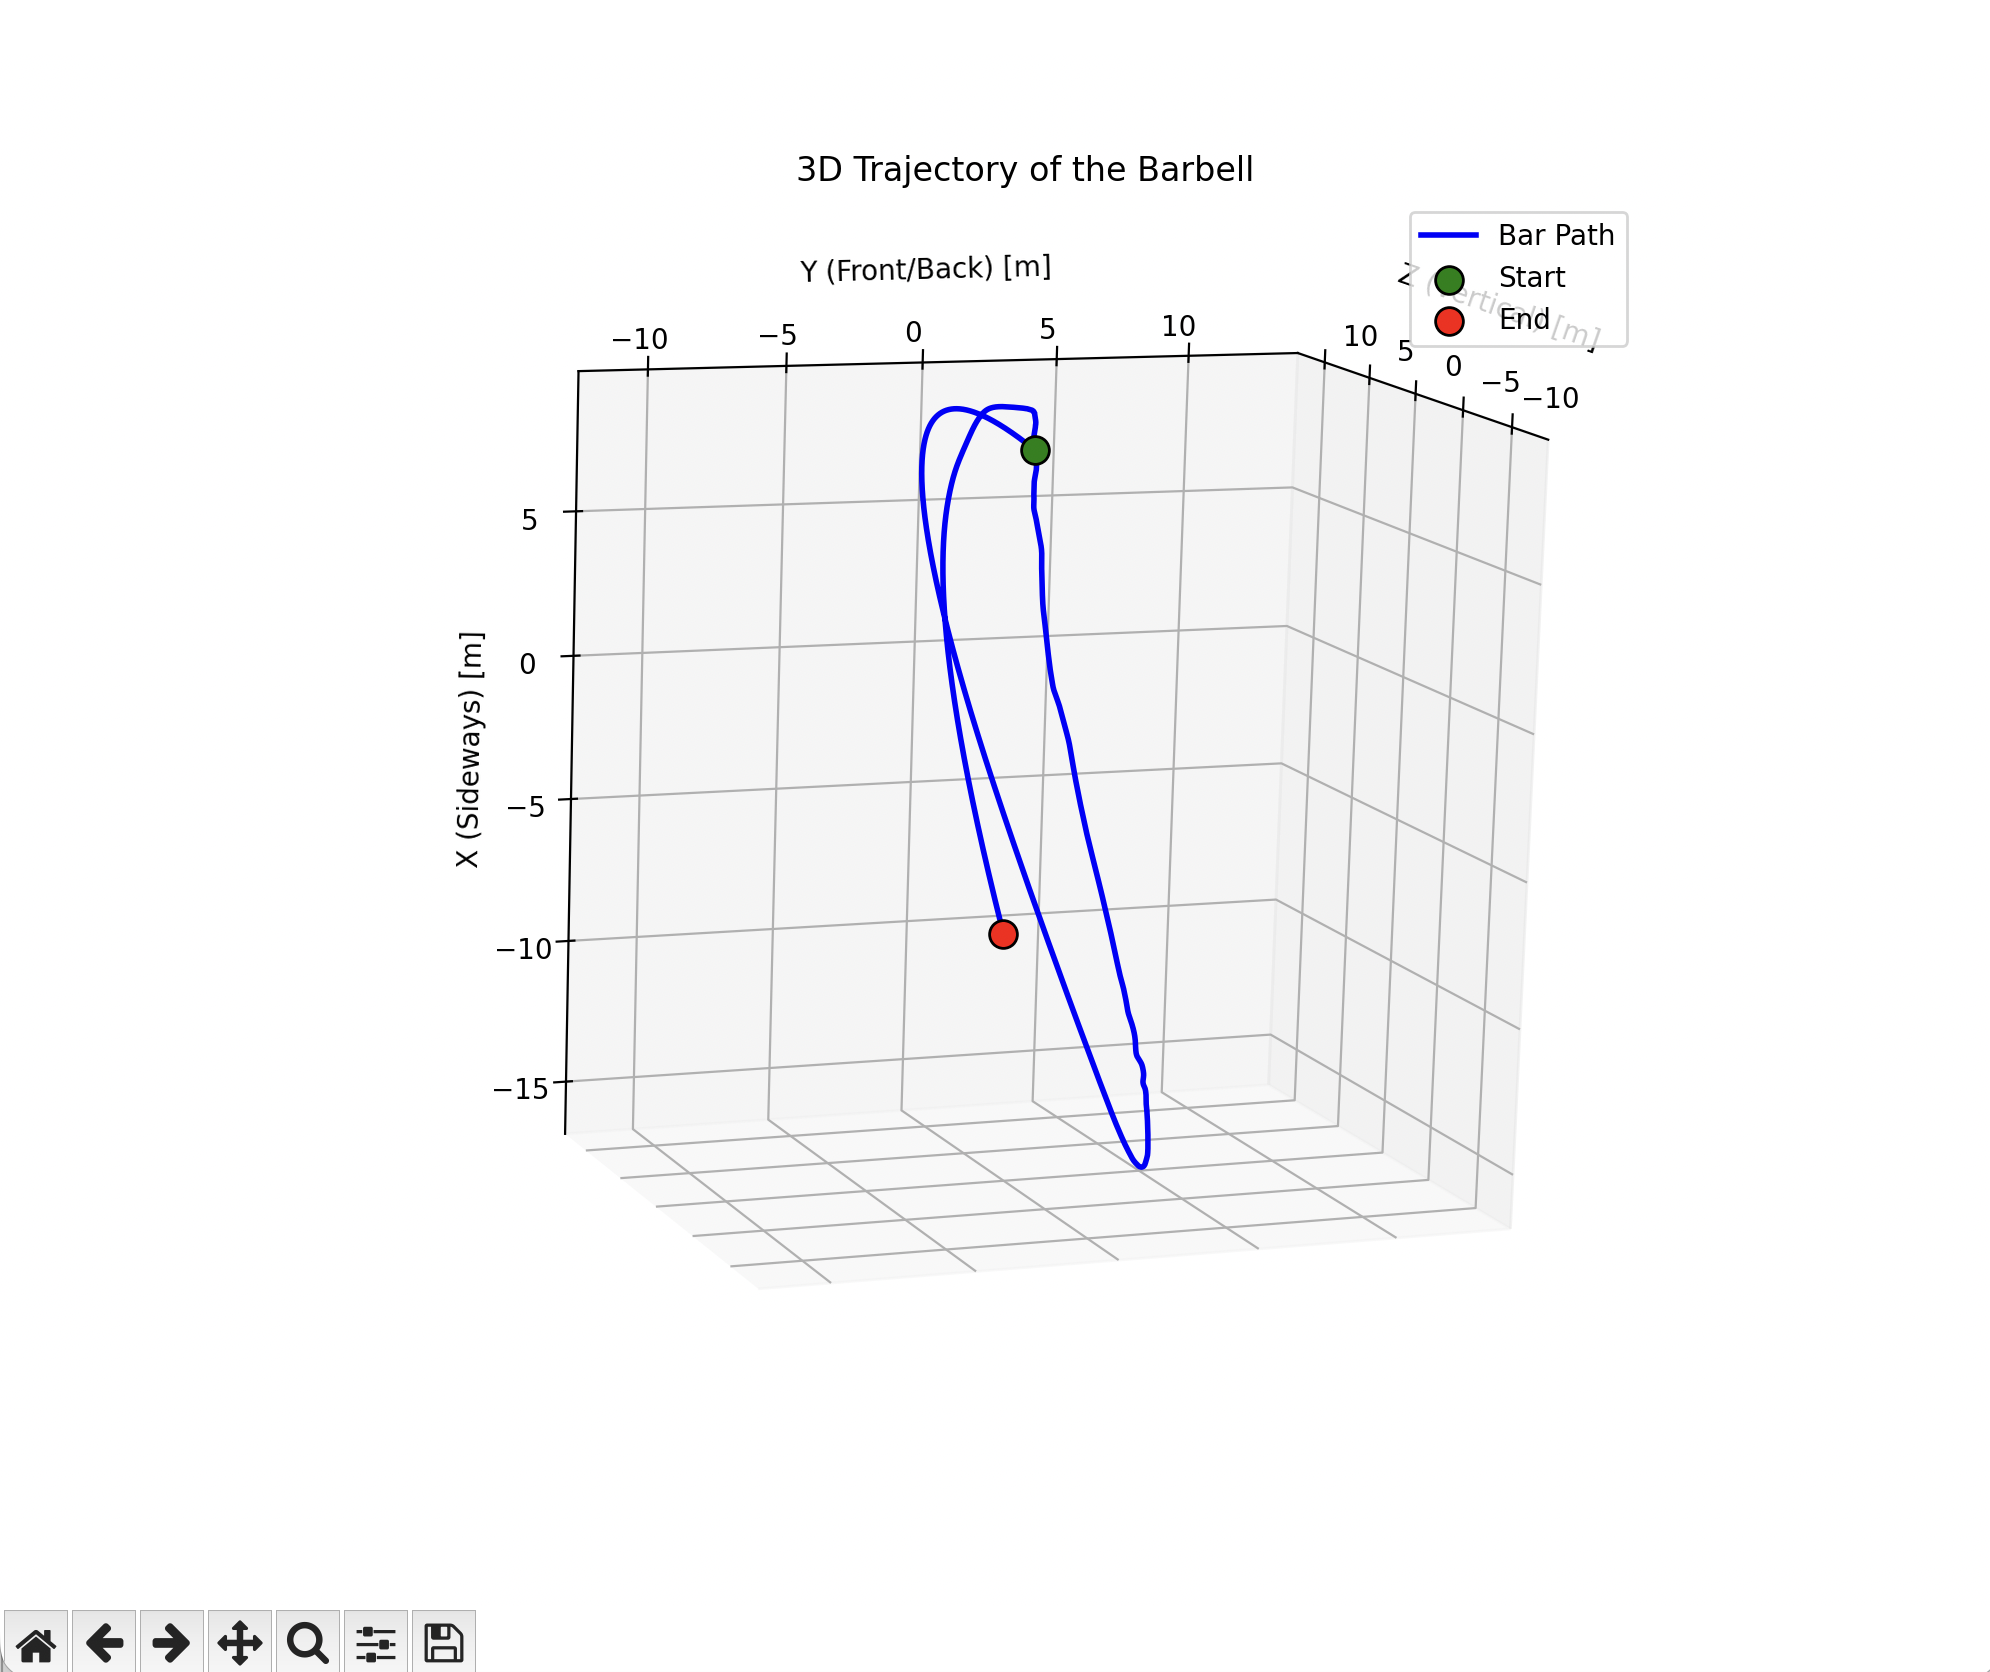
\includegraphics[width=12cm]{images/Annexes/imu-trajectory.png}
  \caption{Trajectoire 3D de la barre reconstruite par double intégration de l'accélération IMU sur un mouvement de squat.}
  \label{fig:imu-trajectory}
\end{figure}

\section*{Difficultés rencontrées}

L'approche IMU s'est heurtée à trois difficultés majeures, qui ont finalement motivé le basculement vers une approche basée sur la vision par ordinateur.

\paragraph{Calibration.}
La calibration du capteur s'est révélée laborieuse et peu reproductible entre les différentes sessions. Chaque mise en service nécessitait une procédure manuelle de calibration du magnétomètre (rotations dans les trois axes) et de l'accéléromètre (positionnement statique selon plusieurs orientations). La présence de métal dans l'environnement (rack, disques, barre elle-même) perturbait significativement les mesures du magnétomètre, rendant l'orientation absolue peu fiable malgré la compensation de biais implémentée.

\paragraph{Dérive.}
Le calcul de la vitesse et de la trajectoire par intégration de l'accélération est intrinsèquement sujet à une dérive cumulative : la moindre erreur résiduelle de calibration s'accumule au cours du temps. Bien que \texttt{scipy.signal.detrend} atténue partiellement ce phénomène en supprimant la composante linéaire de la dérive, les erreurs non linéaires persistent (figure~\ref{fig:imu-dashboard}) et produisent des trajectoires qui s'éloignent progressivement de la réalité sur des séries de plusieurs répétitions consécutives, rendant l'analyse multi-répétitions inexploitable.

\begin{figure}[h]
  \centering
  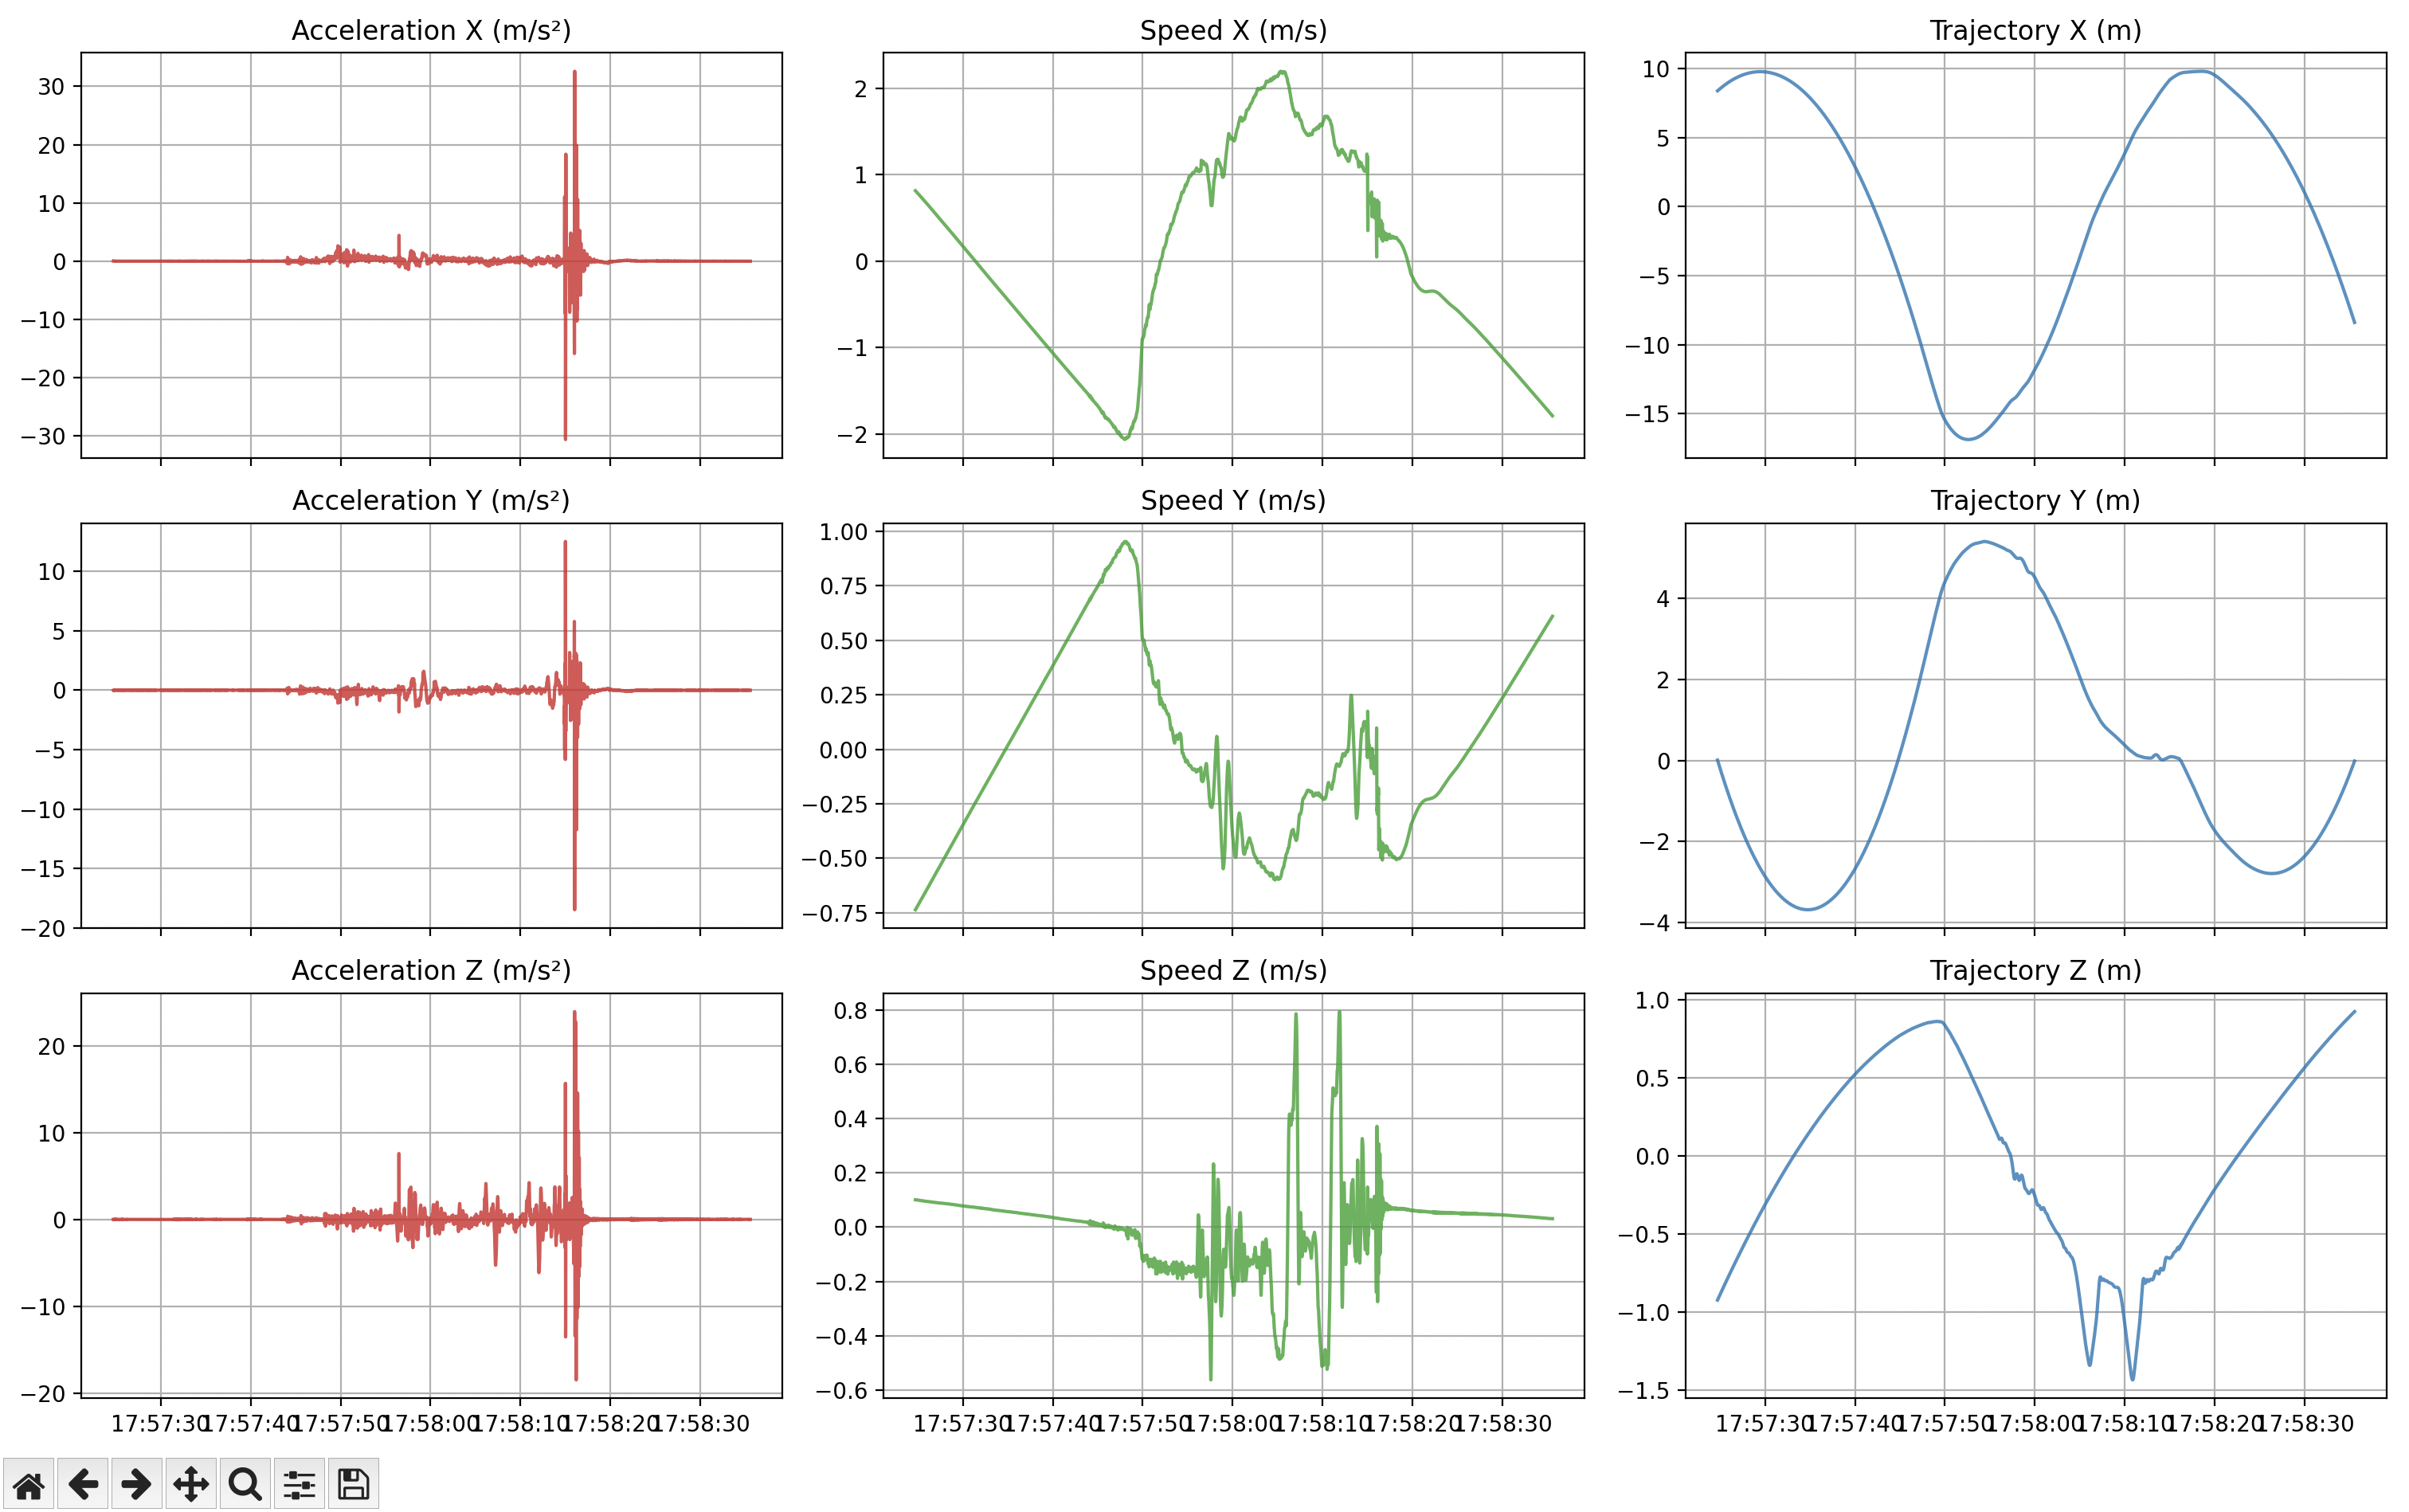
\includegraphics[width=12cm]{images/Annexes/imu-dashboard.png}
  \caption{Dashboard des données IMU : accélération, vitesse et trajectoire par axe (X, Y, Z) sur un enregistrement de squat.}
  \label{fig:imu-dashboard}
\end{figure}

\paragraph{Bruit.}
Les vibrations transmises à la barre durant les phases de mise en place et les micro-tremblements de l'individu généraient un bruit haute fréquence sur l'accéléromètre (figure~\ref{fig:imu-dashboard}). Un filtrage passe-bas atténuait ce bruit mais introduisait un lissage des pics caractéristiques du mouvement, dégradant la précision de détection des transitions de phase du mouvement.

\section*{Bilan}

Bien que l'IMU offre un accès direct aux paramètres cinématiques de la barre, son utilisation pratique en conditions d'entraînement s'est révélée trop contraignante : calibration fastidieuse à chaque session, dérive cumulative limitant la durée d'enregistrement exploitable, et bruit nécessitant un filtrage qui dégrade les transitions de phase. Surtout, l'IMU ne fournit aucune information sur la \emph{posture} de l'individu, qui constitue pourtant l'objet central de l'analyse biomécanique en force athlétique. Ces constats ont conduit à abandonner l'approche instrumentale au profit d'une approche \emph{markerless} basée sur la vision par ordinateur, capable de capturer simultanément la cinématique de la barre (via les keypoints des poignets) et la posture complète de l'individu depuis une simple caméra.


% ===============================================
% ANNEXE B
% ===============================================
\chapter{Interface web de visualisation} \label{ann:web-interface}

Cette annexe présente les fonctionnalités de l'interface web
développée pour explorer les reconstructions 3D produites par
le pipeline.

\section*{Vue d'ensemble}

L'interface se compose de trois zones distinctes : la zone de visualisation 3D centrale affichant le maillage MHR de l'athlète, le panneau de contrôle en bas à droite permettant de naviguer trame par trame et de choisir l'angle de vue caméra, et le panneau de métriques biomécaniques en haut à droite affichant les indicateurs de conformité aux critères IPF en temps réel. Les figures~\ref{fig:web-squat}, \ref{fig:web-bench} et~\ref{fig:web-deadlift} illustrent l'interface pour chacun des trois mouvements de référence.

\section*{Métriques biomécaniques calculées}

Pour chaque mouvement, les métriques suivantes sont calculées en temps réel à partir des keypoints 3D exportés par SAM 3D Body :

\paragraph{Squat.}
Profondeur IPF (hanche sous le niveau du genou sur au moins une trame), inclinaison maximale du buste sur l'ensemble de la séquence, asymétrie maximale des hanches, distance cumulée parcourue par chaque main.

\paragraph{Développé couché.}
Verrouillage des coudes (angle épaule--coude--poignet > 160° atteint en fin de mouvement), angle minimal des coudes, symétrie des poignets, distance cumulée parcourue par chaque main.

\paragraph{Soulevé de terre.}
Verrouillage des genoux, position des épaules par rapport aux hanches sur l'axe de profondeur (critères IPF), inclinaison maximale du buste, asymétrie maximale des hanches, angle minimal des hanches, distance cumulée parcourue par chaque main.

\section*{Captures d'écran représentatives}

\begin{figure}[H]
  \centering
  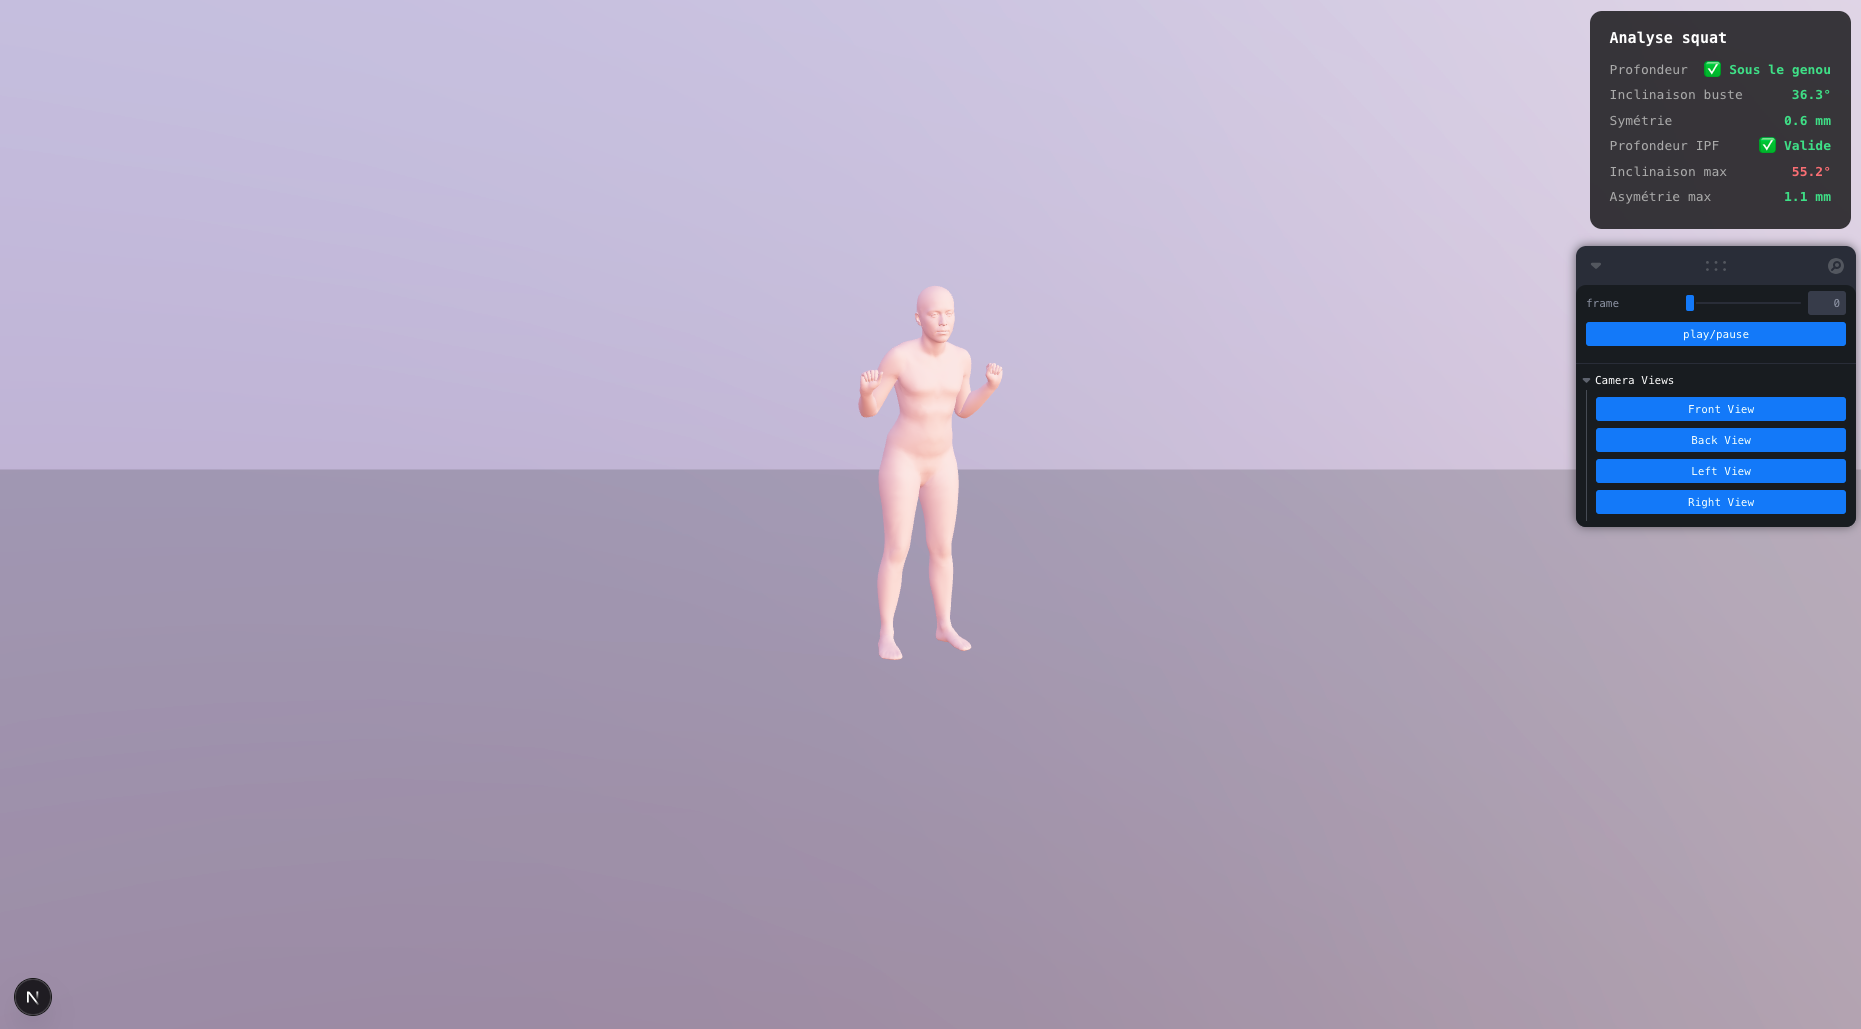
\includegraphics[width=0.95\textwidth]{images/Annexes/web_overview_squat.png}
  \caption{Interface web - squat. La profondeur IPF est validée (hanche sous le genou). L'inclinaison du buste est de 36,3° sur la trame courante, avec un maximum de 55,2° sur l'ensemble de la séquence.}
  \label{fig:web-squat}
\end{figure}

\begin{figure}[H]
  \centering
  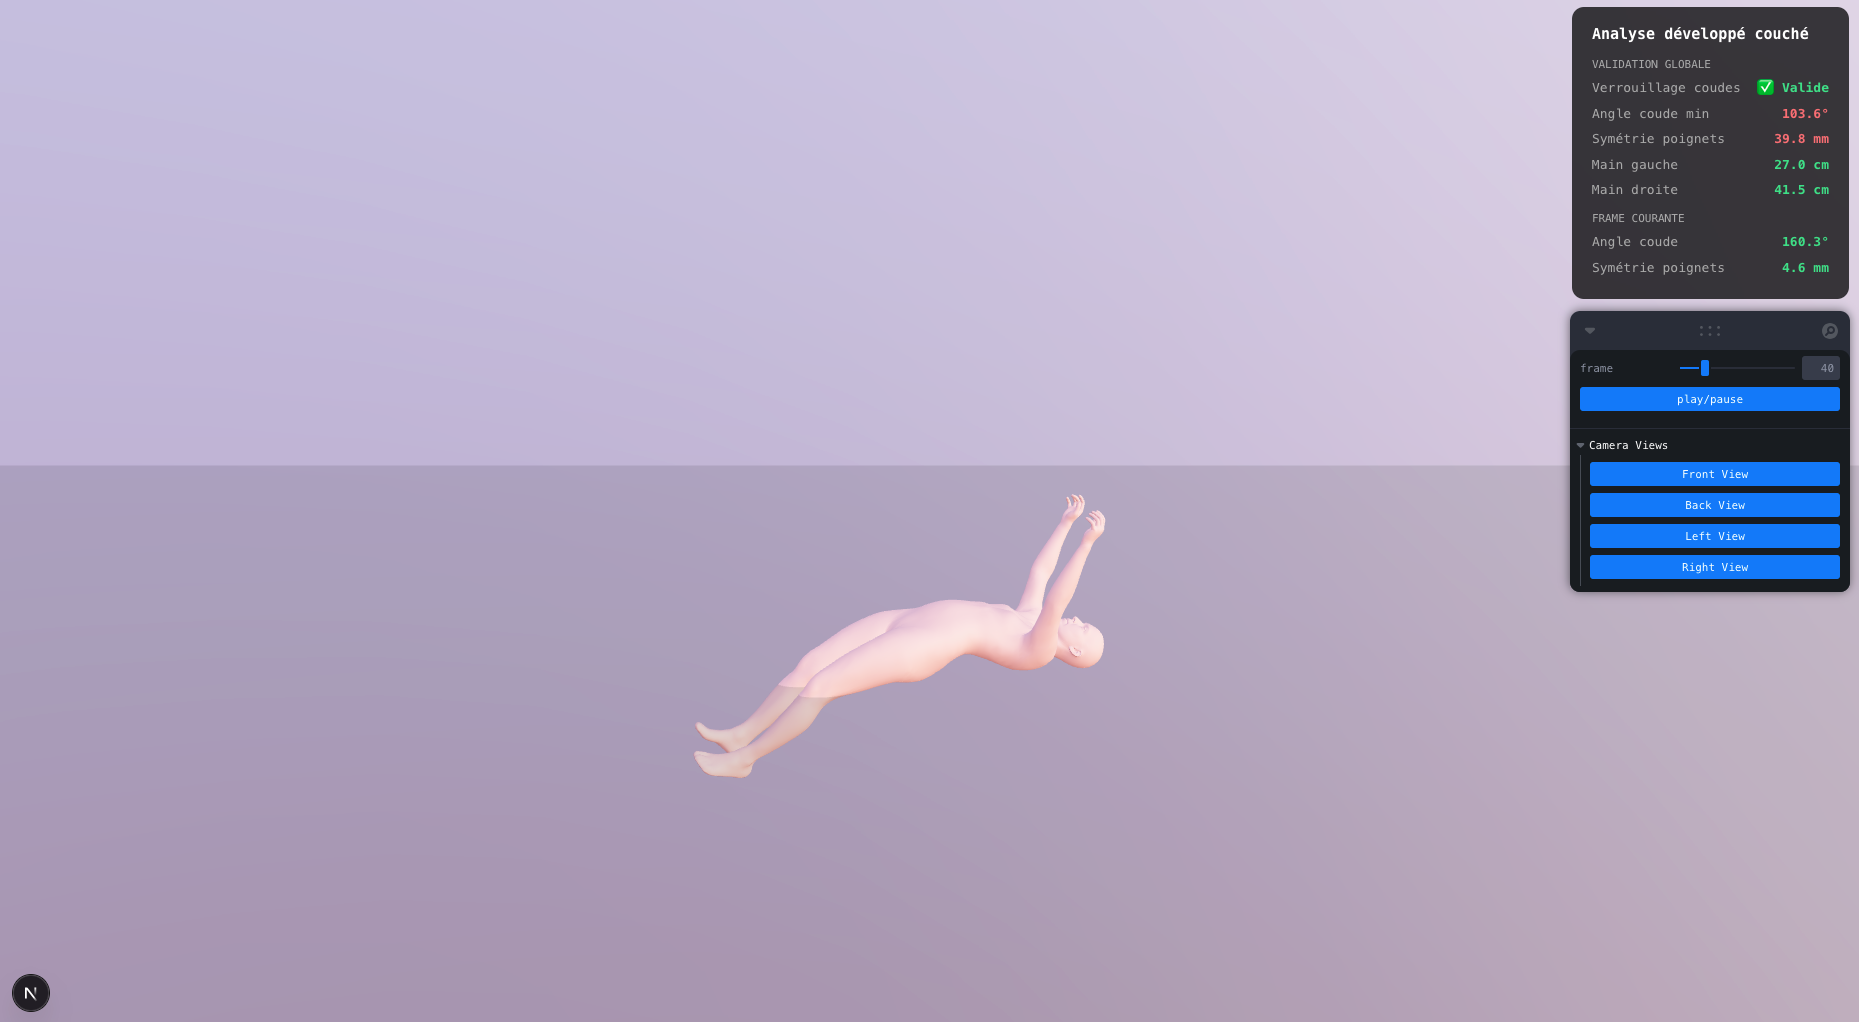
\includegraphics[width=0.95\textwidth]{images/Annexes/web_overview_bench.png}
  \caption{Interface web - développé couché. Le verrouillage des coudes est validé (angle de 160,3° atteint en fin de mouvement). L'angle minimal des coudes de 103,6° correspond à la descente de la barre.}
  \label{fig:web-bench}
\end{figure}

\begin{figure}[H]
  \centering
  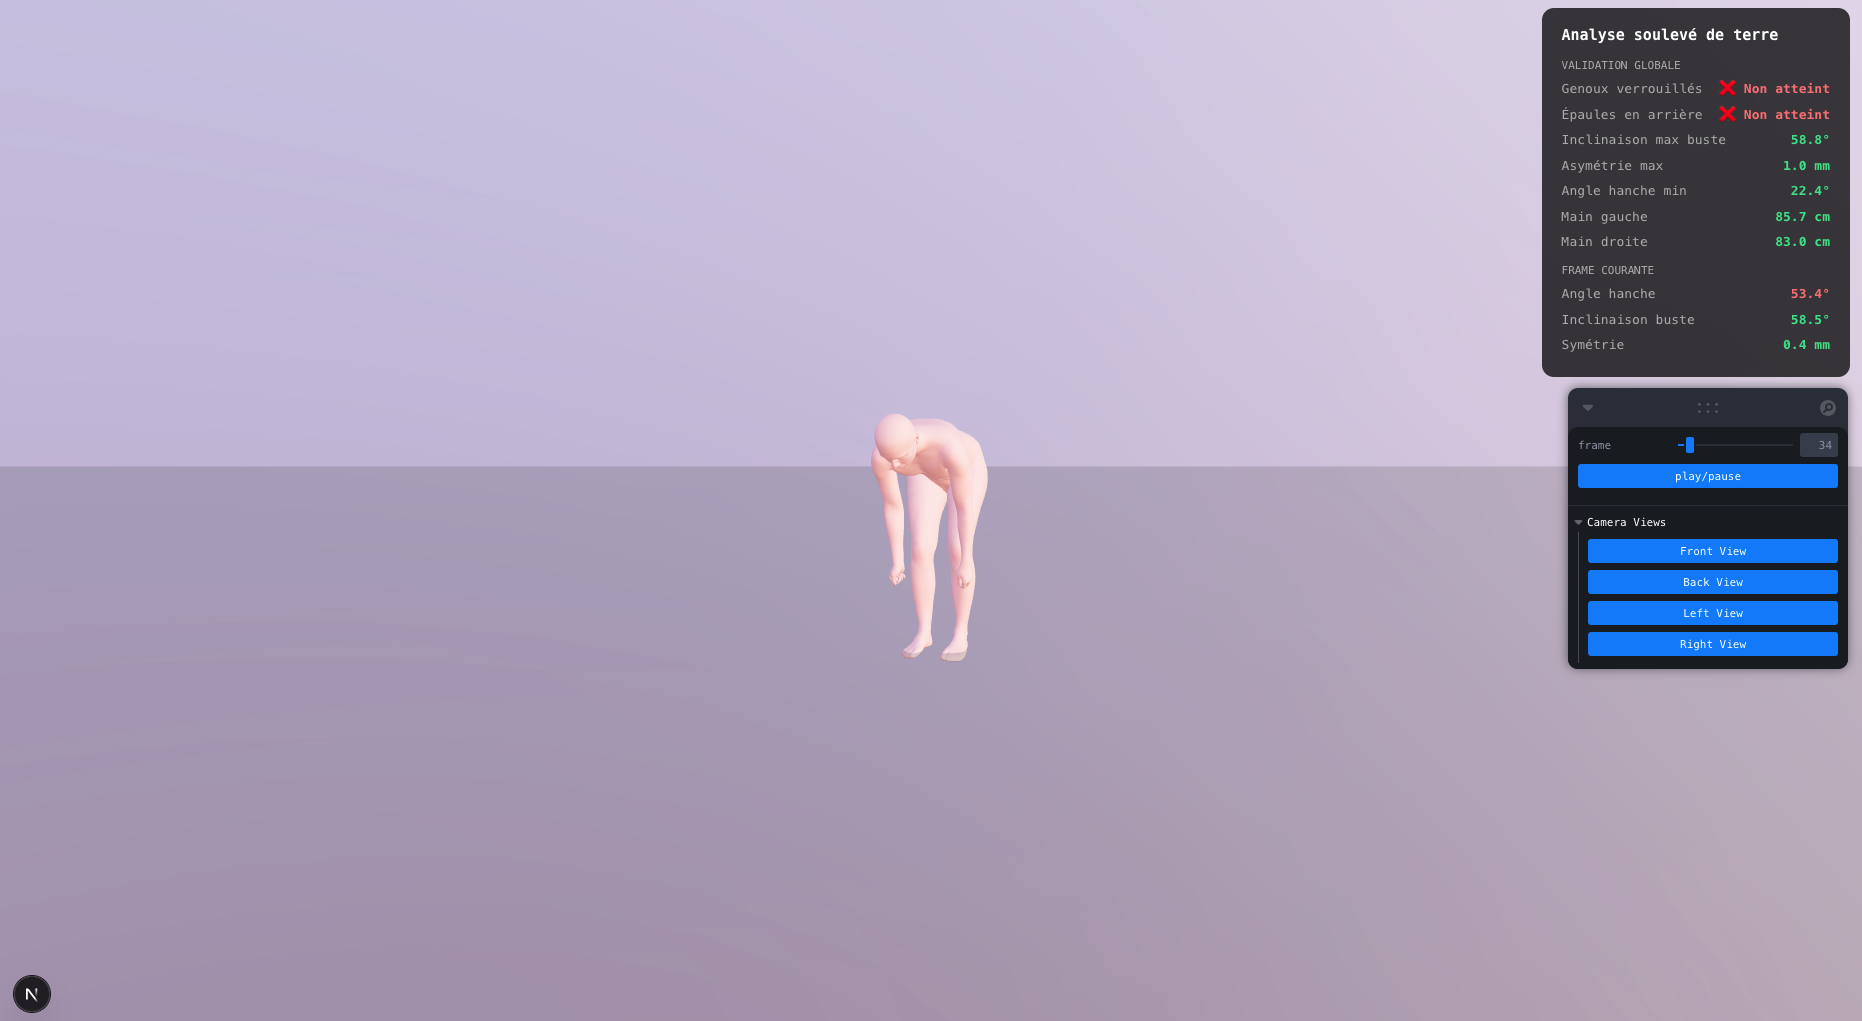
\includegraphics[width=0.95\textwidth]{images/Annexes/web_overview_deadlift.png}
  \caption{Interface web - soulevé de terre. Les critères IPF de verrouillage des genoux et d'épaules en arrière ne sont pas atteints sur cette trame, correspondant à la phase de tirage avec une inclinaison du buste de 58,5°.}
  \label{fig:web-deadlift}
\end{figure}


% ===============================================
% ANNEXE C
% ===============================================
\chapter{Composition détaillée du dataset} \label{ann:dataset-details}

Cette annexe présente la composition détaillée du dataset constitué
pour le fine-tuning de TACO.

\section*{Vidéos sources}

Le tableau~\ref{tab:dataset-detail} recense l'ensemble des vidéos
sources avec leurs métadonnées.

\begin{table}[h]
  \centering
  \small
  \begin{tabular}{llllllll}
    \hline
    \textbf{ID} & \textbf{Sujet} & \textbf{Exercice} & \textbf{Résolution} & \textbf{Durée (s)} & \textbf{FPS} & \textbf{Partition} \\
    \hline
    IMG\_0001 & S01 & Squat    & 540x720 & 2.5 & 30 & Train \\
    IMG\_0002 & S01 & Deadlift & 360x480 & 4.4 & 30 & Train \\
    IMG\_0003 & S01 & Bench    & 360x480 & 2.5 & 30 & Train \\
    IMG\_0004 & S02 & Squat    & 360x480 & 4.6 & 30 & Train \\
    IMG\_0005 & S02 & Deadlift & 360x480 & 7.5 & 30 & Val   \\
    IMG\_0006 & S02 & Deadlift & 360x480 & 3.1 & 30 & Val   \\
    IMG\_0007 & S03 & Deadlift & 540x960 & 13.3 & 30 & Train \\
    IMG\_0008 & S03 & Bench    & 360x640 & 13.4 & 30 & Val   \\
    IMG\_0009 & S03 & Bench    & 540x960 & 11.1 & 30 & Exclu (occlusion réelle) \\
    IMG\_0010 & S04 & Squat    & 3840x2160 & 13.2 & 25 & Train \\
    IMG\_0011 & S03 & Squat    & 3840x2160 & 27.1 & 25 & Exclu (occlusion réelle) \\
    IMG\_0012 & S04 & Deadlift & 3840x2160 & 24.7 & 25 & Train \\
    IMG\_0013 & S04 & Deadlift & 3840x2160 & 23.5 & 25 & Train \\
    IMG\_0014 & S04 & Bench    & 3840x2160 & 16.6 & 25 & Train \\
    IMG\_0015 & S05 & Squat    & 1280x720 & 21.2 & 30 & Train \\
    IMG\_0016 & S05 & Squat    & 1280x720 & 23.5 & 30 & Train \\
    IMG\_0017 & S05 & Deadlift & 1280x720 & 24.3 & 30 & Train \\
    IMG\_0018 & S05 & Deadlift & 1280x720 & 18.8 & 30 & Train \\
    IMG\_0019 & S06 & Deadlift & 540x960 & 8.8 & 30 & Val   \\
    IMG\_0020 & S07 & Squat    & 540x960 & 6.7 & 30 & Train \\
    IMG\_0021 & S07 & Deadlift & 360x640 & 8.4 & 30 & Train \\
    IMG\_0022 & S07 & Bench    & 360x640 & 10.5 & 30 & Train \\
    IMG\_0023 & S08 & Deadlift & 360x640 & 18.0 & 29.776 & Train \\
    IMG\_0024 & S08 & Squat    & 360x640 & 16.1 & 29.737 & Train \\
    IMG\_0025 & S08 & Bench    & 360x640 & 12.4 & 29.752 & Train \\
    \hline
    IMG\_0026 & S09 & Squat    & 536x954 & 17.7 & 30 & Test  \\
    IMG\_0027 & S09 & Bench    & 356x634 & 15.3 & 30 & Test  \\
    IMG\_0028 & S09 & Deadlift & 360x640 & 7.0 & 30 & Test  \\
    \hline
    IMG\_0098 & S03 & Squat    & 2922x1644 & 6.6 & 25 & Exclu (occlusion réelle) \\
    IMG\_0099 & S03 & Deadlift & 3840x2160 & 4.3 & 25 & Exclu (occlusion réelle) \\
    \hline
  \end{tabular}
  \caption{Composition du dataset : métadonnées des vidéos sources. Les vidéos du jeu de données de test (S09) ont été reçues après la réalisation du fine-tuning et n'apparaissent pas dans les partitions d'entraînement ou de validation.}
  \label{tab:dataset-detail}
\end{table}

\section*{Distribution par mouvement et par sujet}

La figure~\ref{fig:dataset-distribution} présente la distribution des séquences d'entraînement par mouvement et par sujet.

\begin{figure}[ht]
  \centering
  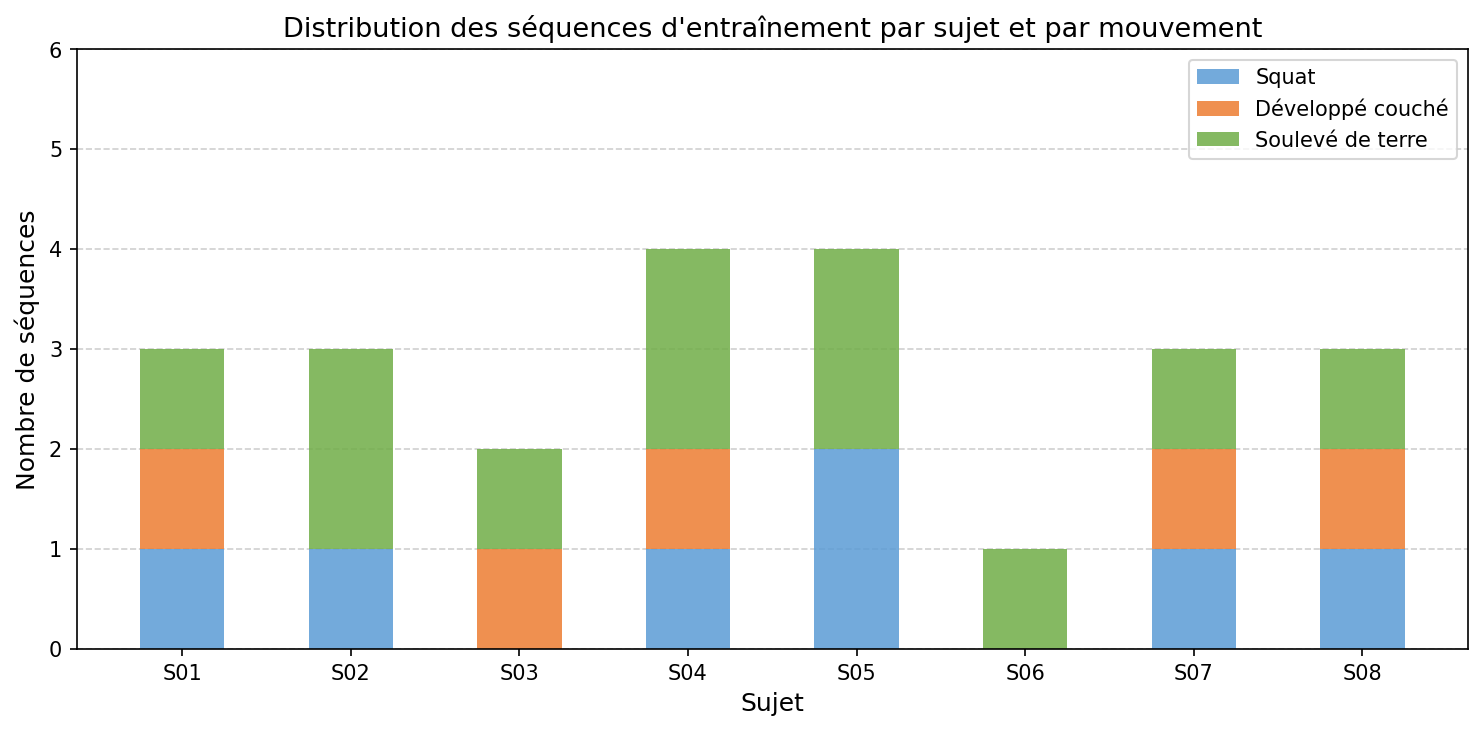
\includegraphics[width=12cm]{images/Annexes/dataset_distribution.png}
  \caption{Distribution des séquences du dataset d'entraînement par mouvement et par sujet.}
  \label{fig:dataset-distribution}
\end{figure}

\section*{Banque d'occlusions synthétiques}

La figure~\ref{fig:occluders-bank} présente l'ensemble des occlusions utilisées pour la génération synthétique des occlusions du dataset d'entraînement.

\begin{figure}[ht]
  \centering
  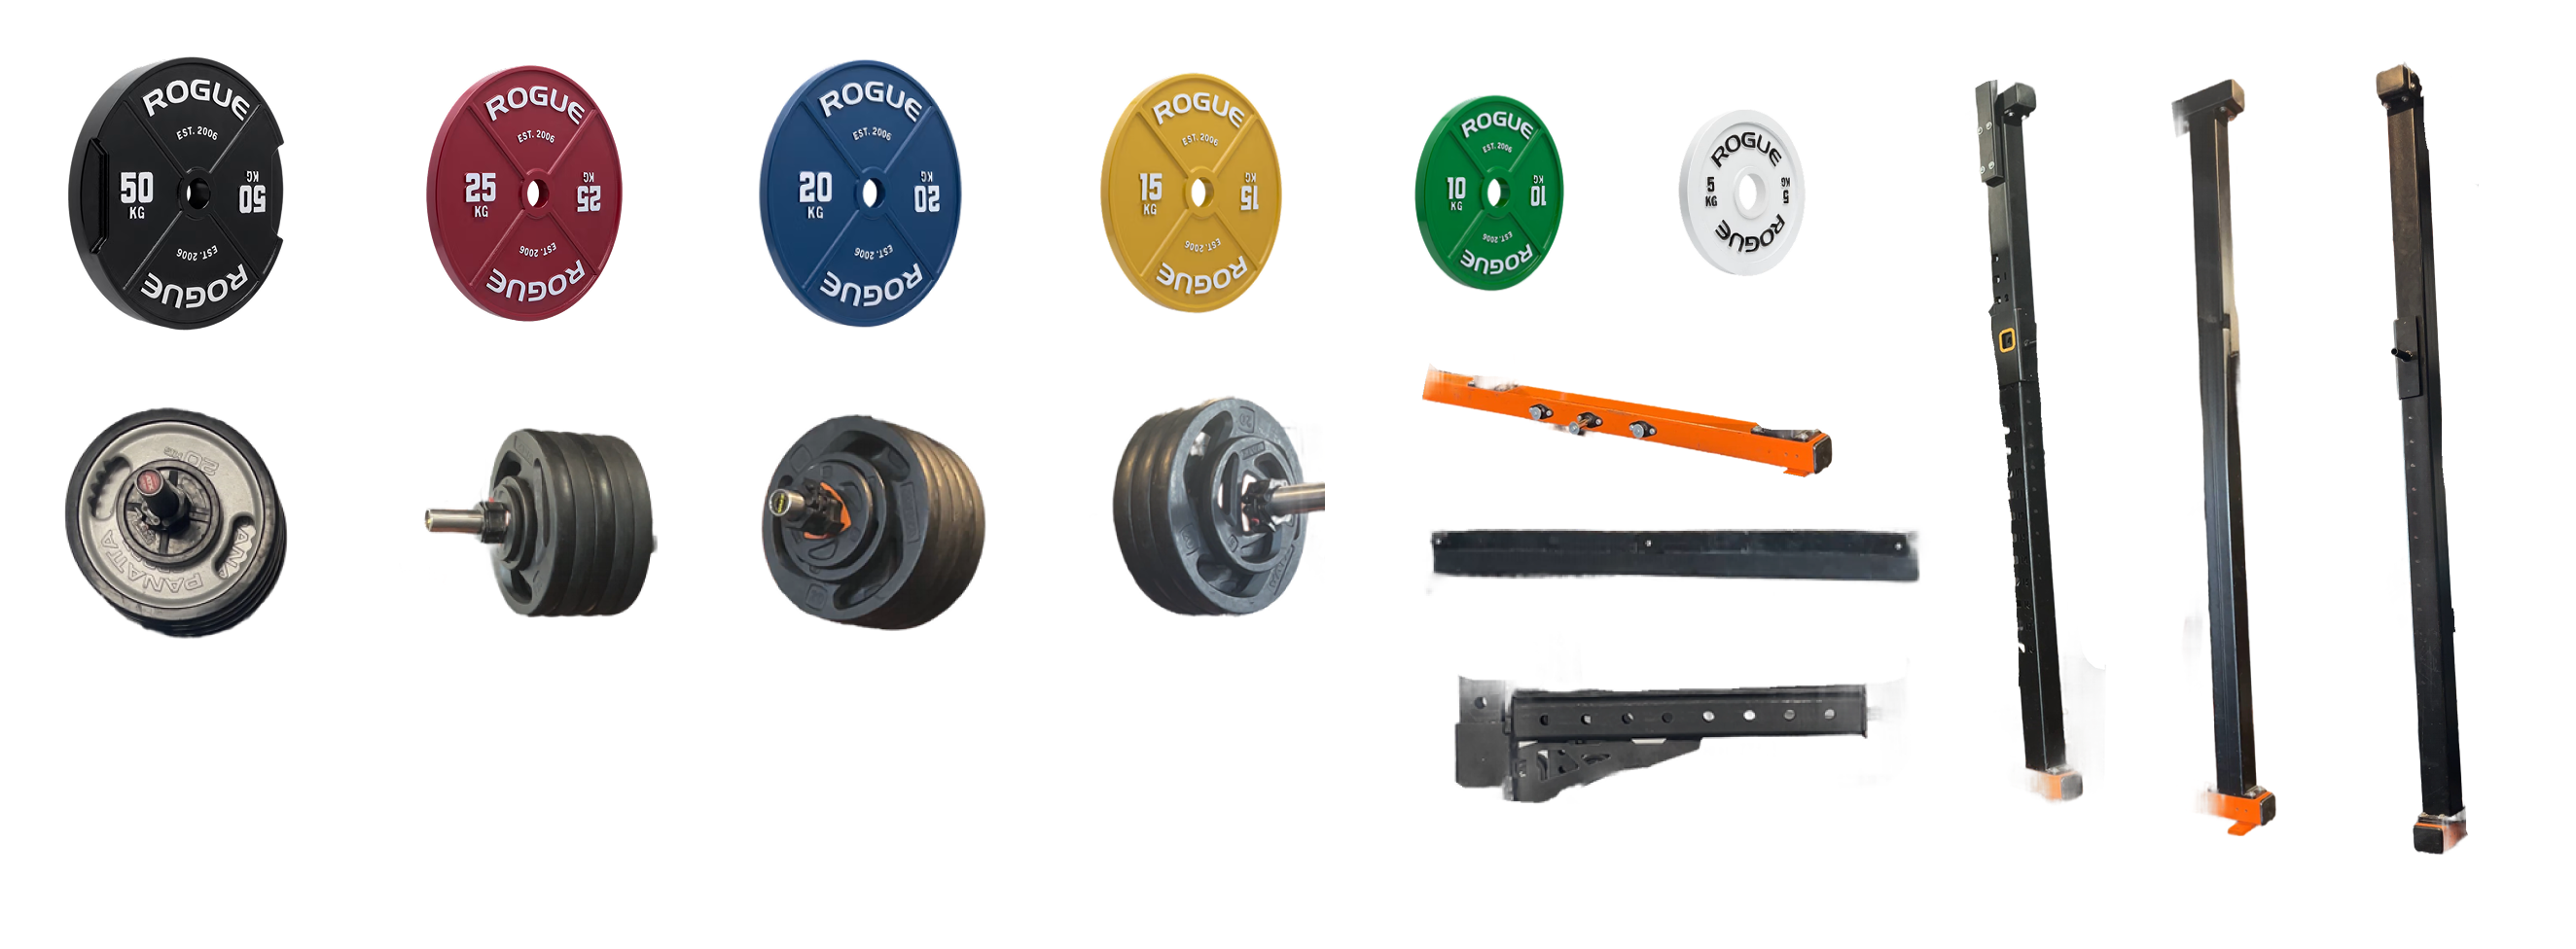
\includegraphics[width=14cm]{images/Annexes/occluders.png}
  \caption{Banque d'occlusions synthétiques utilisés pour la génération des occlusions du dataset de fine-tuning : disques IPF calibrés, disques de salle commerciale, configurations multi-disques et racks à squat.}
  \label{fig:occluders-bank}
\end{figure}


% ===============================================
% ANNEXE D
% ===============================================
\chapter{Charte de traitement des données personnelles} \label{ann:rgpd}

Cette annexe reproduit la charte RGPD établie pour la collecte des vidéos auprès des sujets volontaires.

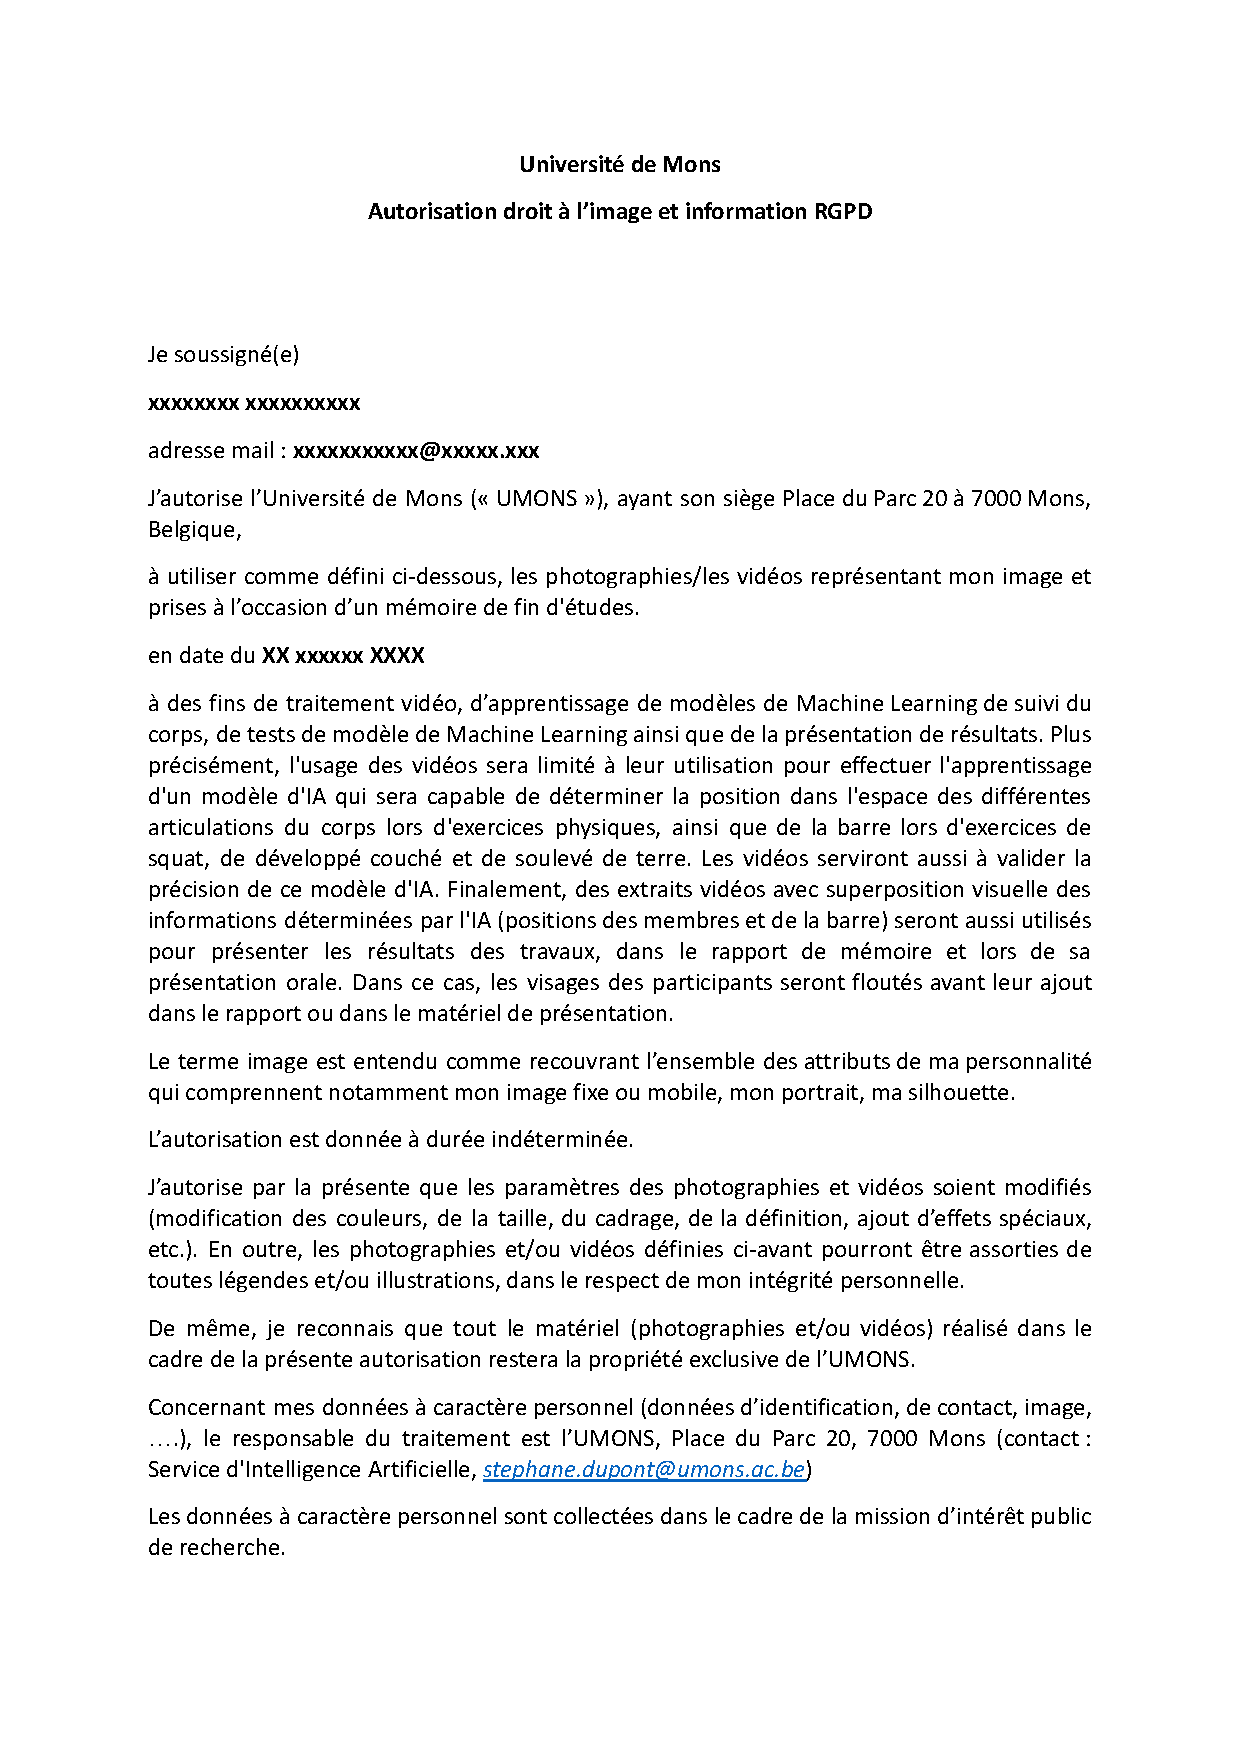
\includepdf[pages=-, scale=0.9, pagecommand={}, offset=0 -1cm]{images/Annexes/RGPD-Template.pdf}

% ===============================================
% ANNEXE E
% ===============================================
\chapter{Configuration du fine-tuning LoRA} \label{ann:lora-config}

Cette annexe détaille la configuration utilisée pour le fine-tuning LoRA de TACO, complétant les informations synthétiques fournies au chapitre~\ref{ch_four}.

\section*{Couches ciblées par LoRA}

La stratégie \texttt{time\_lora} cible 248 modules répartis en cinq catégories, tous liés au traitement temporel du UNet de Stable Video Diffusion. Le tableau~\ref{tab:lora-layers} présente une synthèse par catégorie.

\begin{table}[ht]
  \centering
  \begin{tabular}{lrrr}
    \hline
    \textbf{Type de module} & \textbf{Nb couches} &
    \textbf{Params / couche} & \textbf{Params total} \\
    \hline
    Embedding temporel (\texttt{time\_embed}) & 2
      & 25\,600 -- 40\,960 & 66\,560 \\
    Embedding de timestep (\texttt{emb\_layers}) & 22
      & 25\,600 -- 40\,960 & $\approx$ 700\,000 \\
    Position temporelle (\texttt{time\_pos\_embed}) & 24
      & 25\,600 -- 102\,400 & $\approx$ 2\,100\,000 \\
    Auto-attention temporelle (\texttt{attn1}) & 48
      & 10\,240 -- 40\,960 & $\approx$ 1\,700\,000 \\
    Cross-attention temporelle (\texttt{attn2}) & 48
      & 10\,240 -- 40\,960 & $\approx$ 1\,600\,000 \\
    Feed-forward temporel (\texttt{ff}, \texttt{ff\_in}) & 104
      & 25\,600 -- 184\,320 & $\approx$ 5\,500\,000 \\
    \hline
    \textbf{Total} & \textbf{248} & -- & \textbf{11\,700\,000} \\
    \hline
  \end{tabular}
  \caption{Synthèse des 248 couches ciblées par la stratégie \texttt{time\_lora} avec rang $r = 16$. Les modules d'attention spatiale, le VAE et les embeddings de conditionnement (CLIP) sont intégralement gelés et ne figurent pas dans ce tableau.}
  \label{tab:lora-layers}
\end{table}

\section*{Statistiques d'utilisation des ressources}

\begin{figure}[H]
  \centering

  % GPU Utilisation
  \begin{subfigure}[t]{0.48\textwidth}
    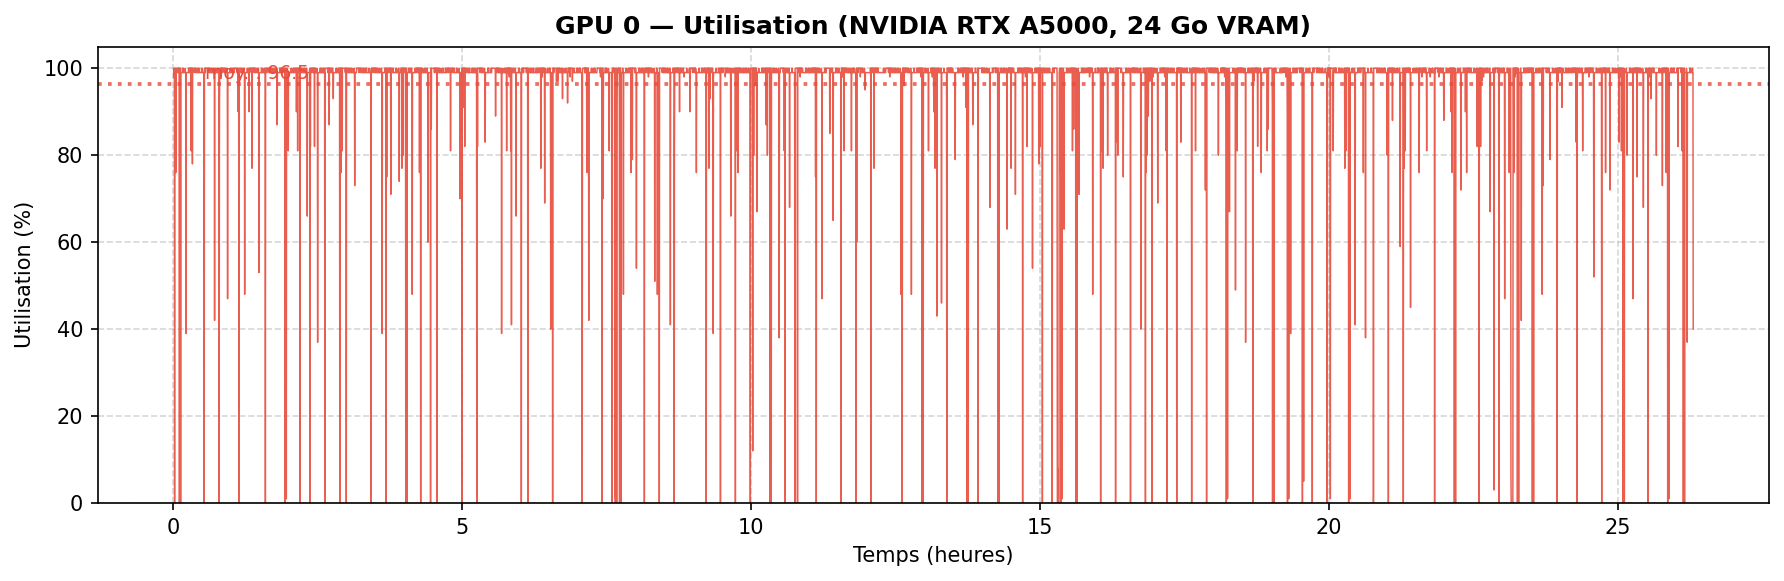
\includegraphics[width=\textwidth]{images/Annexes/gpu0_utilisation.png}
    \caption{GPU 0 — Utilisation (\%)}
  \end{subfigure}
  \hfill
  \begin{subfigure}[t]{0.48\textwidth}
    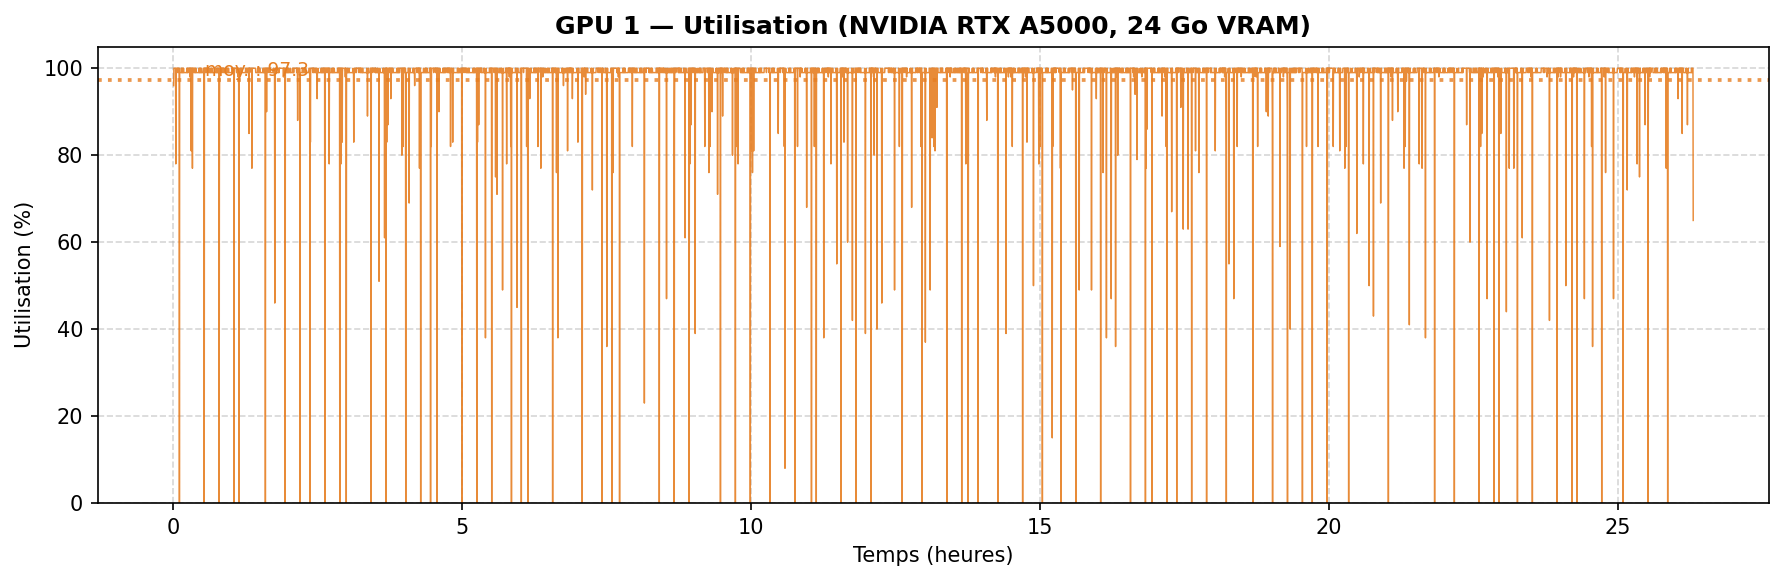
\includegraphics[width=\textwidth]{images/Annexes/gpu1_utilisation.png}
    \caption{GPU 1 — Utilisation (\%)}
  \end{subfigure}

  \vspace{0.5em}

  % GPU Température
  \begin{subfigure}[t]{0.48\textwidth}
    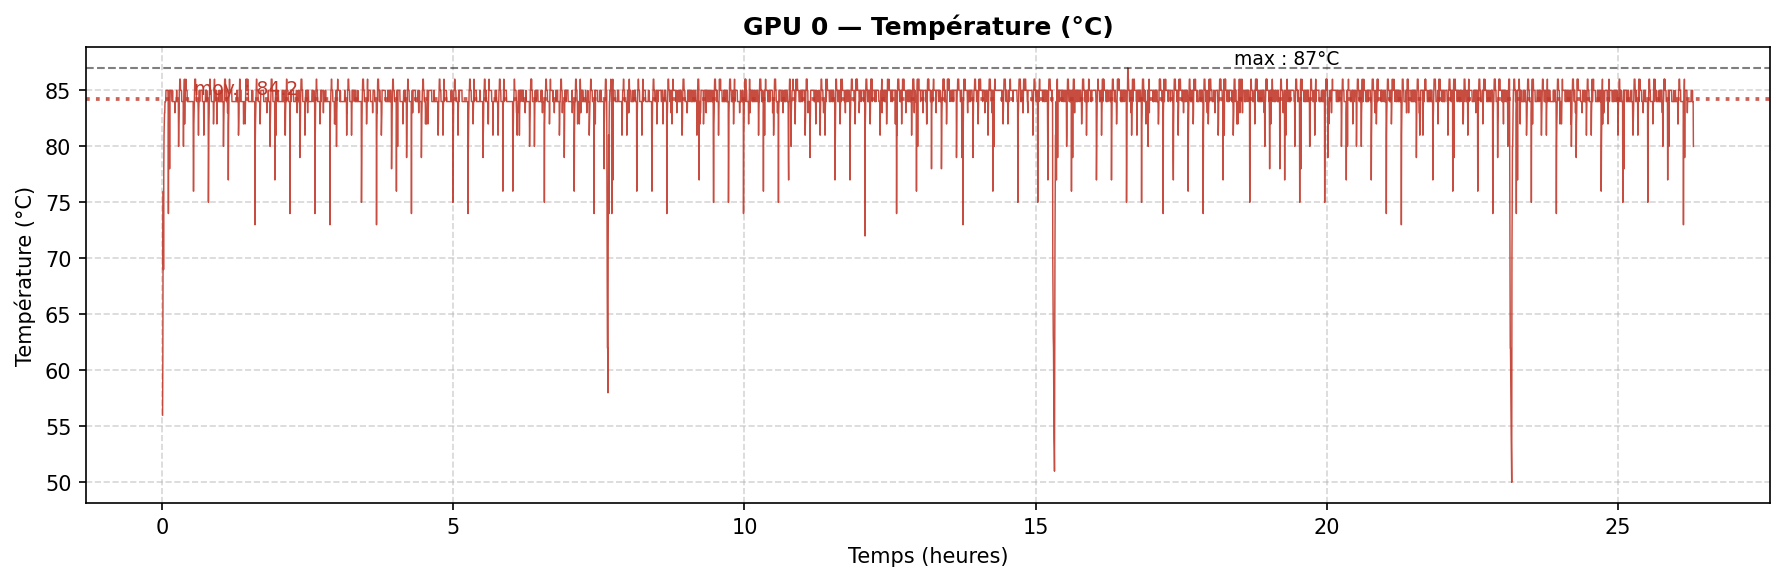
\includegraphics[width=\textwidth]{images/Annexes/gpu0_temperature.png}
    \caption{GPU 0 — Température (°C)}
  \end{subfigure}
  \hfill
  \begin{subfigure}[t]{0.48\textwidth}
    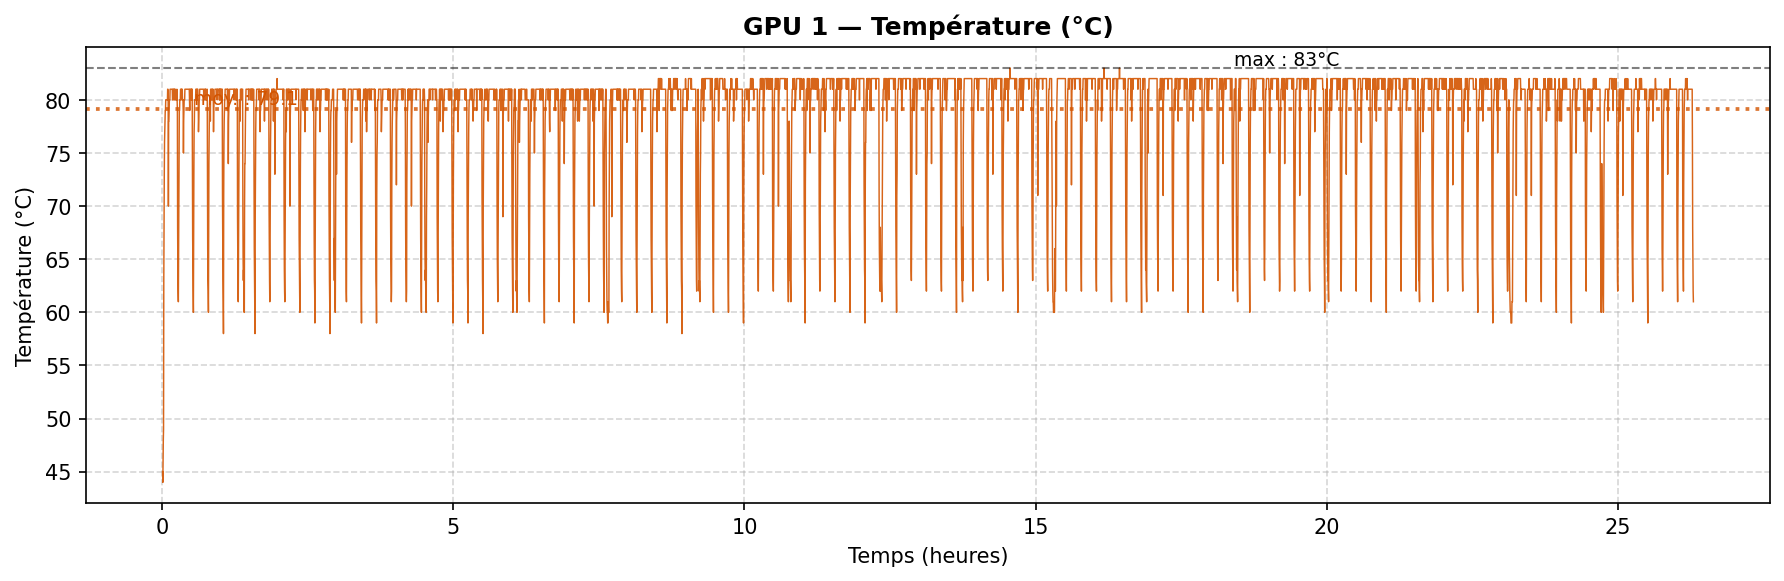
\includegraphics[width=\textwidth]{images/Annexes/gpu1_temperature.png}
    \caption{GPU 1 — Température (°C)}
  \end{subfigure}

  \vspace{0.5em}

  % RAM et CPU
  \begin{subfigure}[t]{0.48\textwidth}
    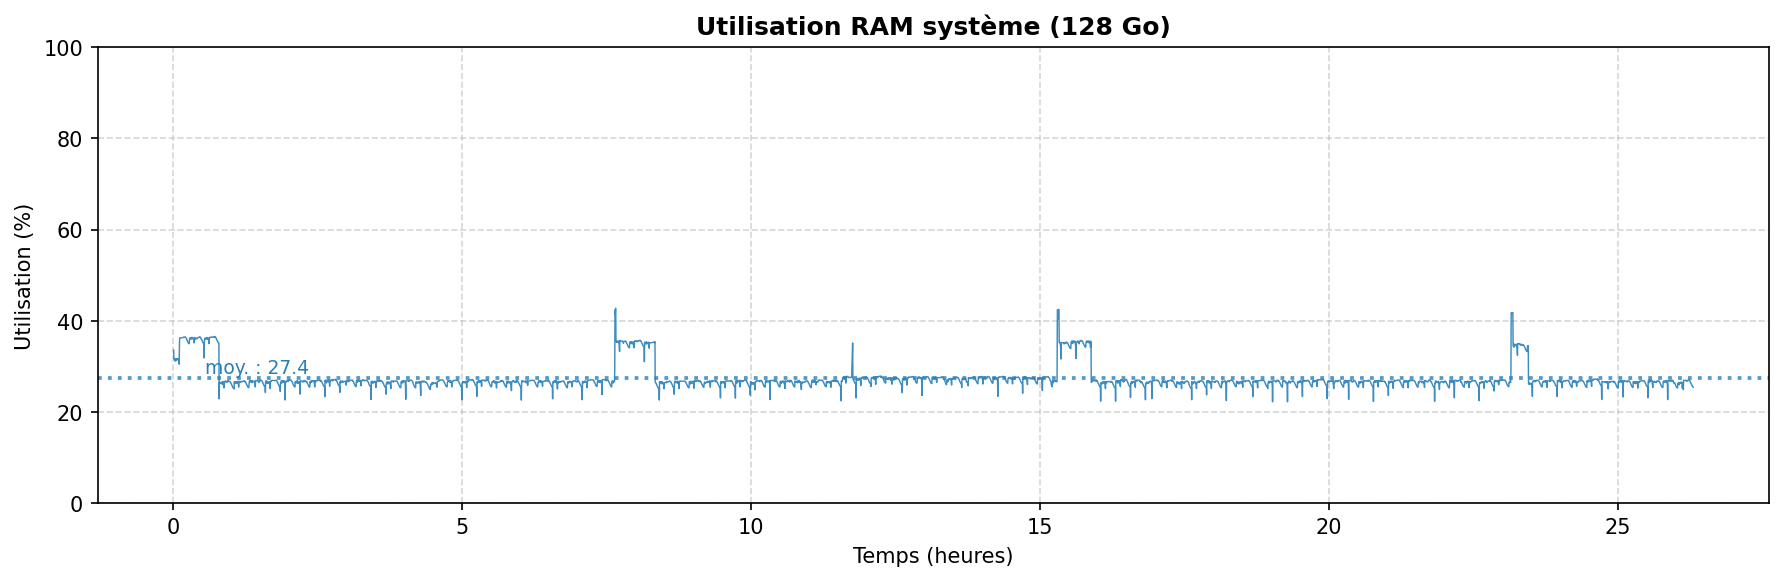
\includegraphics[width=\textwidth]{images/Annexes/ram_utilisation.png}
    \caption{Utilisation RAM système (128~Go)}
  \end{subfigure}
  \hfill
  \begin{subfigure}[t]{0.48\textwidth}
    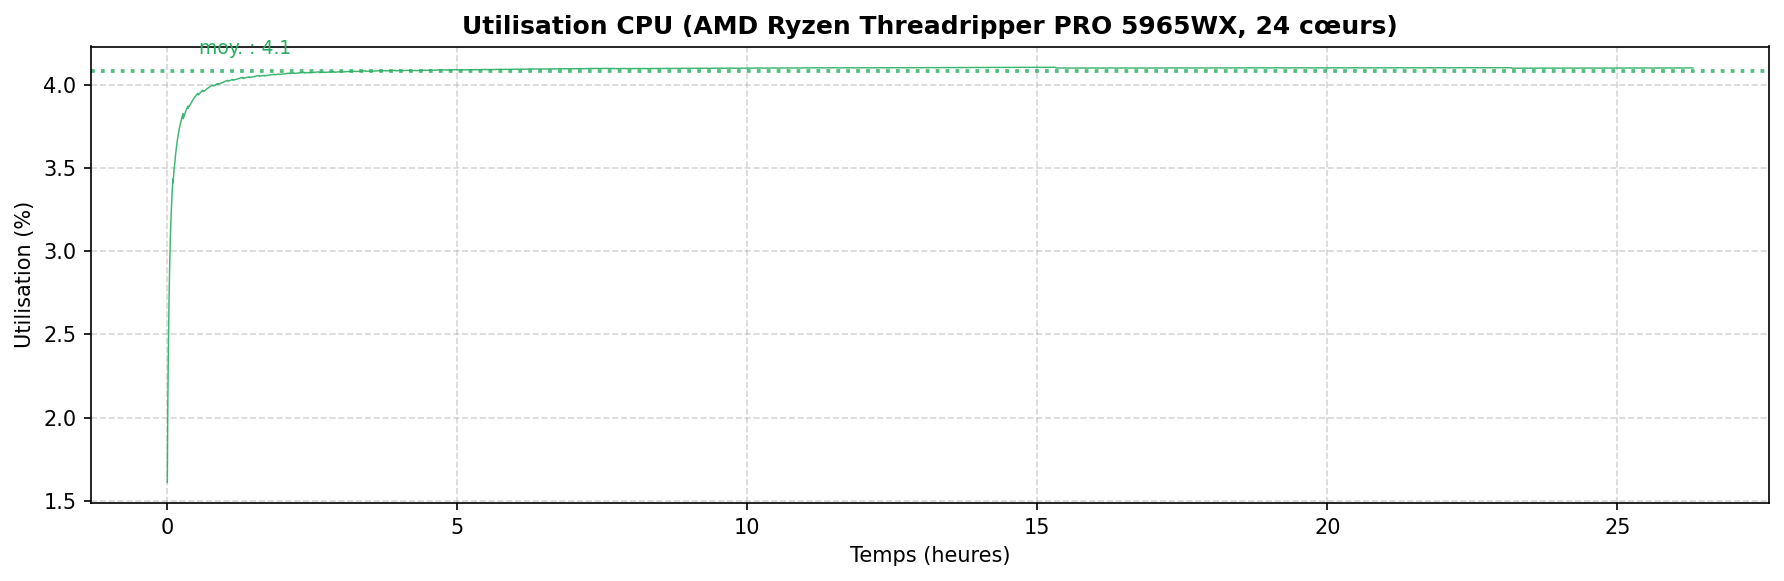
\includegraphics[width=\textwidth]{images/Annexes/cpu_utilisation.png}
    \caption{Utilisation CPU (24 cœurs)}
  \end{subfigure}

  \caption{Utilisation des ressources matérielles durant le fine-tuning LoRA sur 26,3 heures. Les deux GPU atteignent une utilisation moyenne de 96,5\,\% et 97,3\,\% respectivement, confirmant la saturation effective du matériel disponible. La RAM système reste modérément sollicitée (27,4\,\% en moyenne), le goulot d'étranglement étant la mémoire VRAM.}
  \label{fig:system-usage}
\end{figure}


% ===============================================
% ANNEXE F
% ===============================================
\chapter{Reproductibilité et code source} \label{ann:reproducibility}

\section*{Dépôt de code}

L'intégralité du code source du pipeline est disponible publiquement sur GitHub :

\begin{center}
  \url{https://github.com/nicolasdelp/MEMOIRE-Master-en-Sciences-Informatiques}

  \vspace{0.5em}
  \qrcode[height=2.5cm]{https://github.com/nicolasdelp/MEMOIRE-Master-en-Sciences-Informatiques}
  
  \vspace{0.3em}
  {\small \textit{Scanner pour accéder au dépôt GitHub}}
\end{center}

\section*{Structure du projet}

\begin{lstlisting}[style=tree]
/
|-- code/
|   |-- checkpoints/    (checkpoints des modeles)
|   |-- logs/           (logs d'entrainement)
|   |-- models/         (SAM3, MoGe, TACO, SAM 3D Body)
|   |-- scripts/        (differents scripts d'execution)
|   `-- web/            (interface de visualisation)
|-- data/
|   |-- assets/         (occlusions et ressources visuelles)
|   |-- datasets/       (dataset de fine-tuning)
|   |-- inputs/         (videos brutes)
|   `-- outputs/        (resultats intermediaires)
|-- report/
|   |-- chapters/       (chapitres LaTeX)
|   |-- images/         (figures et illustrations)
|   |-- memoire.bib     (bibliographie)
|   |-- memoire.pdf     (document compile)
|   `-- memoire.tex     (fichier principal)
|-- models.lock         (versions des checkpoints)
|-- pixi.toml           (dependances et taches)
`-- README.md
\end{lstlisting}

\section*{Instructions d'installation et d'utilisation}

L'ensemble des instructions détaillées est disponible dans le fichier \texttt{README.md} du dépôt. Les étapes principales sont résumées ci-dessous.

\paragraph{Prérequis matériels (minimum).}~\\
\begin{itemize}
  \item 2 GPU NVIDIA RTX A5000 (24~Go VRAM chacun) ou équivalent
  \item 128~Go de RAM système
  \item Ubuntu 22.04 LTS, CUDA 12.2
\end{itemize}

\paragraph{1. Téléchargement des checkpoints.}~\\

Installer l'outil CLI HuggingFace puis s'authentifier :

\begin{lstlisting}[style=bash]
curl -LsSf https://hf.co/cli/install.sh | bash
hf auth login
\end{lstlisting}

Télécharger chaque checkpoint dans son dossier dédié
(voir tableau~\ref{tab:checkpoints} pour les liens) :

\begin{lstlisting}[style=bash]
cd code/checkpoints/sam3/
hf download facebook/sam3 sam3.pt --local-dir .

cd code/checkpoints/moge/
hf download Ruicheng/moge-2-vitl model.pt --local-dir .

cd code/checkpoints/taco/
wget https://huggingface.co/datasets/JasonAplp/TACO/\
resolve/main/checkpoints/last.ckpt
hf download Nicolasdelp/TACO-LoRA-Powerlifting \
lora.ckpt --local-dir .

cd code/checkpoints/sam_3d_body/
hf download facebook/sam-3d-body-vith model.ckpt --local-dir .
curl -OL https://github.com/facebookresearch/MHR/\
releases/download/v1.0.0/assets.zip
unzip -p assets.zip assets/mhr_model.pt > mhr_model.pt
rm assets.zip
\end{lstlisting}

\paragraph{2. Installation de Pixi et du dataset.}~\\

\begin{lstlisting}[style=bash]
wget -qO- https://pixi.sh/install.sh | sh
pixi self-update
\end{lstlisting}

Télécharger et extraire le dataset :

\begin{lstlisting}[style=bash]
cd data/
for tar_file in outputs/IMG_*.tar; do
    tar -xf "$tar_file" -C outputs/
done
\end{lstlisting}

\paragraph{3. Lancer le pipeline principal.}~\\

\begin{lstlisting}[style=bash]
pixi run main-pipeline
\end{lstlisting}

\paragraph{4. Lancer l'interface web de visualisation.}~\\

Télécharger les maillages 3D précalculés :

\begin{lstlisting}[style=bash]
cd code/web/public/
hf download Nicolasdelp/Dataset-TFE-Web \
--repo-type=dataset --local-dir .
\end{lstlisting}

Installer Node.js (voir \url{https://nodejs.org/en/download}),
puis lancer l'application :

\begin{lstlisting}[style=bash]
cd code/web/
npm run dev
\end{lstlisting}

\paragraph{5. Reproduire le fine-tuning LoRA.}~\\

\begin{lstlisting}[style=bash]
cd code/models/taco/
conda env create -f environment.yml
conda activate taco
bash train_continue.sh
\end{lstlisting}

\section*{Checkpoints des modèles}

Les checkpoints des différents modèles sont hébergés séparément en raison de leur taille. Le tableau~\ref{tab:checkpoints} recense les liens de téléchargement pour chaque composant du pipeline.

\begin{table}[h]
  \centering
  \small
  \begin{tabular}{ll}
    \hline
    \textbf{Modèle / Ressource} & \textbf{Lien} \\
    \hline
    SAM3 & \url{https://huggingface.co/facebook/sam3} \\
    OpenCLIP (vocabulaire) & \url{https://huggingface.co/spaces/LanguageBind/} \\
                           & \url{LanguageBind/resolve/main/open_clip/} \\
                           & \url{bpe_simple_vocab_16e6.txt.gz} \\
    MoGe-2 & \url{https://huggingface.co/Ruicheng/moge-2-vitl} \\
    TACO baseline & \url{https://huggingface.co/datasets/JasonAplp/TACO/} \\
                  & \url{resolve/main/checkpoints/last.ckpt} \\
    TACO-LoRA-Powerlifting & \url{https://huggingface.co/Nicolasdelp/} \\
    (contribution de ce mémoire) & \url{TACO-LoRA-Powerlifting} \\
    SAM 3D Body & \url{https://huggingface.co/facebook/sam-3d-body-vith} \\
    MHR (assets) & \url{https://github.com/facebookresearch/MHR/} \\
                 & \url{releases/download/v1.0.0/assets.zip} \\
    \hline
  \end{tabular}
  \caption{Liens de téléchargement des checkpoints utilisés dans le pipeline.}
  \label{tab:checkpoints}
\end{table}

\section*{Dataset}

Le dataset constitué pour le fine-tuning de TACO est hébergé sur des disques durs à l'Université de Mons, comme indiqué dans la charte RGPD (annexe~\ref{ann:rgpd}).